
%%\documentclass{article}
\documentclass{scrartcl}


%\usepackage{tocloft}  new
\usepackage{cmap}
\usepackage{booktabs}
\usepackage{colortbl}
\usepackage{multirow}
\usepackage{subfloat}
\usepackage{float}
\floatstyle{boxed} 
\restylefloat{figure}

\usepackage{caption}

\usepackage{lipsum}

\usepackage{kpfonts}

\usepackage{polyglossia}
\usepackage{csquotes}
\setdefaultlanguage{english}
%%%%%%%%%%%%%%%% for color
\usepackage{xcolor, colortbl} 
\newcommand{\mc}[2]{\multicolumn{#1}{c}{#2}}
\definecolor{Gray}{gray}{0.85}
\definecolor{LightCyan}{rgb}{0.88,1,1}

\newcolumntype{a}{>{\columncolor{Gray}}c}
\newcolumntype{b}{>{\columncolor{white}}c}
%%%%%%%%%%%%%%%%%%%%%%%%%%
%\usepackage[backend=biber]{biblatex}
\usepackage[backend=biber, style=ieee]{biblatex}
\addbibresource{plana.bib}

\usepackage{graphicx}
\graphicspath{ {images/} }

%%%% the package and hypersetup below make pdf clickable
\usepackage{hyperref}
\hypersetup{
    colorlinks,
    citecolor=black,
    filecolor=black,
    linkcolor=black,
    urlcolor=black
}
\hypersetup{linktocpage}






\begin{document}

\begin{titlepage}


\title{\textsc{\LARGE Bern University of Applied Sciences | BFH }\\[1cm]
\begin{center}
%
\includegraphics[width = 60mm]{logo.JPG}
\end{center}
\textsc{\small Department of Engineering and Information Technology}\\
\textsc{\small Bachelor's Thesis (BTI7321 ) Autumn Semester 2020/21}\\[1cm]
%\textsc{\small Report on  }\\
\textsc{"Planning of the Assignments for Lecturers(PLANA)" Web Application}}
\date{\today}   %% or \date{01 november 2019}
\author{\textit{Author: }Kristina \textsc{Shiryagina} (\texttt{kristina.shiryagina@bfh.ch}) \\
 \textit{Supervisor: } Prof. Marcel \textsc{Pfahrer}  (\texttt{marcel.pfahrer@bfh.ch})\\
 \textit{Expert: }  \textsc{} \\
 }
\maketitle	

\newpage


	
\tableofcontents
\clearpage
\end{titlepage}

%%%%%%%%%% end title page
\setcounter{secnumdepth}{-2}% default for "report" is 2





\section{Acknowledgments}
%%I would like to thank my project supervisor - Prof. Marcel Pfahrer for his advice and guidance. 
%%I would also like to thank Andrei Herasimau for his corrections and Egger Samuel Sebastian for his advice.


\section{Abstract}


\setcounter{secnumdepth}{2}  % to make sections without numbers



\section{Introduction}







%\section{Customer Problem Statement}
%
%\subsection{Problem Statement}


%\**
%A minimum 3-page high-level narrative about your project. The narrative should not be written from the developer’s perspective, describing the features of the planned system.
%Rather, put yourself into a customer’s role, and write your problem statement as if your imagined customer would write it! —Describe the problem that your customer is facing and his or her suggestions about how a software system could help.
%Your problem statement should be based on your project proposal, revised and improved as necessary.
%*\



\subsection{Acronyms}	
\begin{table}[h]

%\begin{center}
\begin{tabular}{ p{2.5cm}| p{9.5cm} }
\rowcolor{LightCyan}
\hline
\textbf{Acronyms} & \textbf{Words} \\
\hline
EF                   &   Entity Framework\\ 
CSS      & Cascading Style Sheet \\ 
KKK      &              345\\ 
\end{tabular}
%\end{center}
\caption{Caption2}
\label{table2}
\end{table}



\subsection{Glossary}
\begin{itemize}


\item \textbf{FURPS+}\cite{eeles2005capturing} is a system for classifying requirements.
\begin{itemize}
\item Functionality
\item Usability
\item Reliability
\item Performance
\item Supportability 
\end{itemize}


\item \textbf{ SignalIR} is a free and open-source software library for Microsoft ASP.NET that allows server code to send asynchronous notifications to client-side web applications. 

\item \textbf{Blazor} is a free and open-source web framework that enables developers to create web apps using C\# and HTML. It is being developed by Microsoft.

\item \textbf{EF Core} 

\item \textbf{HTML} HyperText Markup language


\item \textbf{SQL} Structured Query Language
\item \textbf{JS } JavaScript
\item \textbf{CRUD} Create, read, update and delete
\item \textbf{UI} User Interface
\item \textbf{API} Application Programming Interface 

\item \textbf{MS} Microsoft
\item \textbf{BPMN} Business Process Model and Notation



\end{itemize}
%\section{System Requirements}


\section{System Architecture and System Design}
In project 2 we have started with describing of System architecture and design. In this work we want go deeper into this topic. \\
\section{Creating the Projects}

\subsection{Structure of Projects and Folders}

\subsection{Data Models}

\subsection{Entity Framework Core Packages}

\subsection{Connection String}

\subsection{Creating the Database Context Class}

\subsection{Entity Framework Core Configuration}

\subsection{Database and Entity Framework Core}
Entity Framework(EF) Core is an object-relational mapper (O /RM). It is designed to make writing code for accessing a database quick and intuitive.
There are many good reasons to use EF Core. It supports LINQ queries, change tracking, updates, and schema migrations. EF Core works with many databases, including SQL Database, SQLite, MySQL, PostgreSQL, and Azure Cosmos DB.
book \cite{efa} \cite{ef}

\subsection{The PLANA App's Relational Database}
Our database has many types of relationships we can have in EF Core. The types are:
One-to-many: Lecturer
Many-to-many:
One-To-Many Relationship : 
Lecturer to an Additional Assignment 
Semester to a Additional Assignment
Semester to a Module Run 
Module to a Module Run
Study Branch to a Module
Many-To-Many Relationship :
Lecturers to Semester
Lecturers to Module
Lecturers to Module Run




\subsection{Modeling Types of Database Relationships}
\subsubsection{Many-to-many Relationship }
Creating many-to-many relationship is little bit different from the one-to-many and one-to-one.
We will take as example relation between Lecturer and Module.\\

In EF Core database doesn't directly implement this kind of relationships.
First we have to create class Lecturer and class Module. Then we have to create one more class, we call it LecturersModules. This class links lecturers to their modules. \\
At the LecturerModules class there are two properties, LecturerId and ModuleId. There are both - primary keys and foreign keys, known as a composite key.\cite{efa}


\begin{figure}[H]
\centering
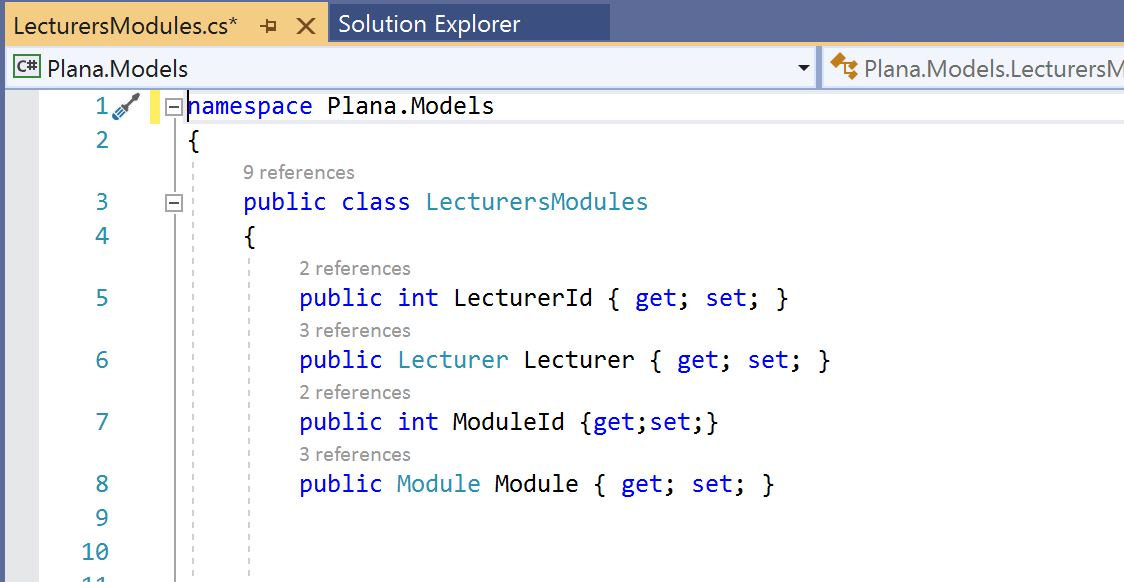
\includegraphics[width=150mm]{report_img/lecturers-modules.JPG}
\caption{The LecturersModules entity class}
\label{blabla}
\end{figure}

 The next step  is adding necessary code to the AppDbContext class. We add 
 \begin{itemize}
 \item \textbf{DbSet<Lecturer>} 
 \item \textbf {DbSet<Module>}
 \item \textbf{DbSet<LecturersModules>}
 \end{itemize}
 
 
 
The Figure 2 below shows this process. In the OnModelCreating method we add
\begin{itemize}
\item\textbf{modelBuilder.Entity<LectuerersModules>().HasKey(x=> new {x.LecturerId, x.ModuleId}};
\end{itemize}


 





\begin{figure}[H]
\centering
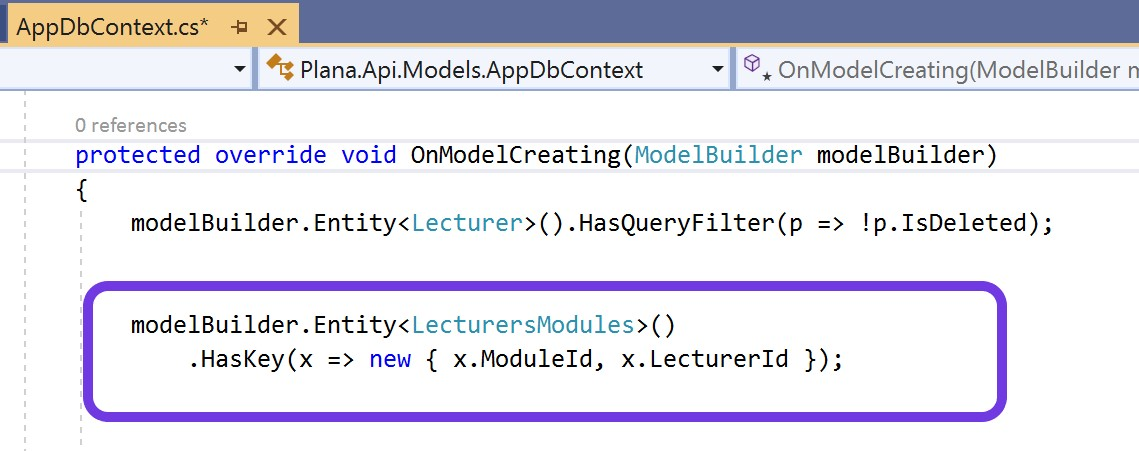
\includegraphics[width=150mm]{report_img/many-to-many.JPG}
\caption{Adding Entity LecturersModules to the AppDbContext class}
\label{blabla}
\end{figure}  
We need write just this and Entity Framework Core will do the correct implementation that we can see then in the migration files. \cite{patrick}

\begin{figure}[H]
\centering
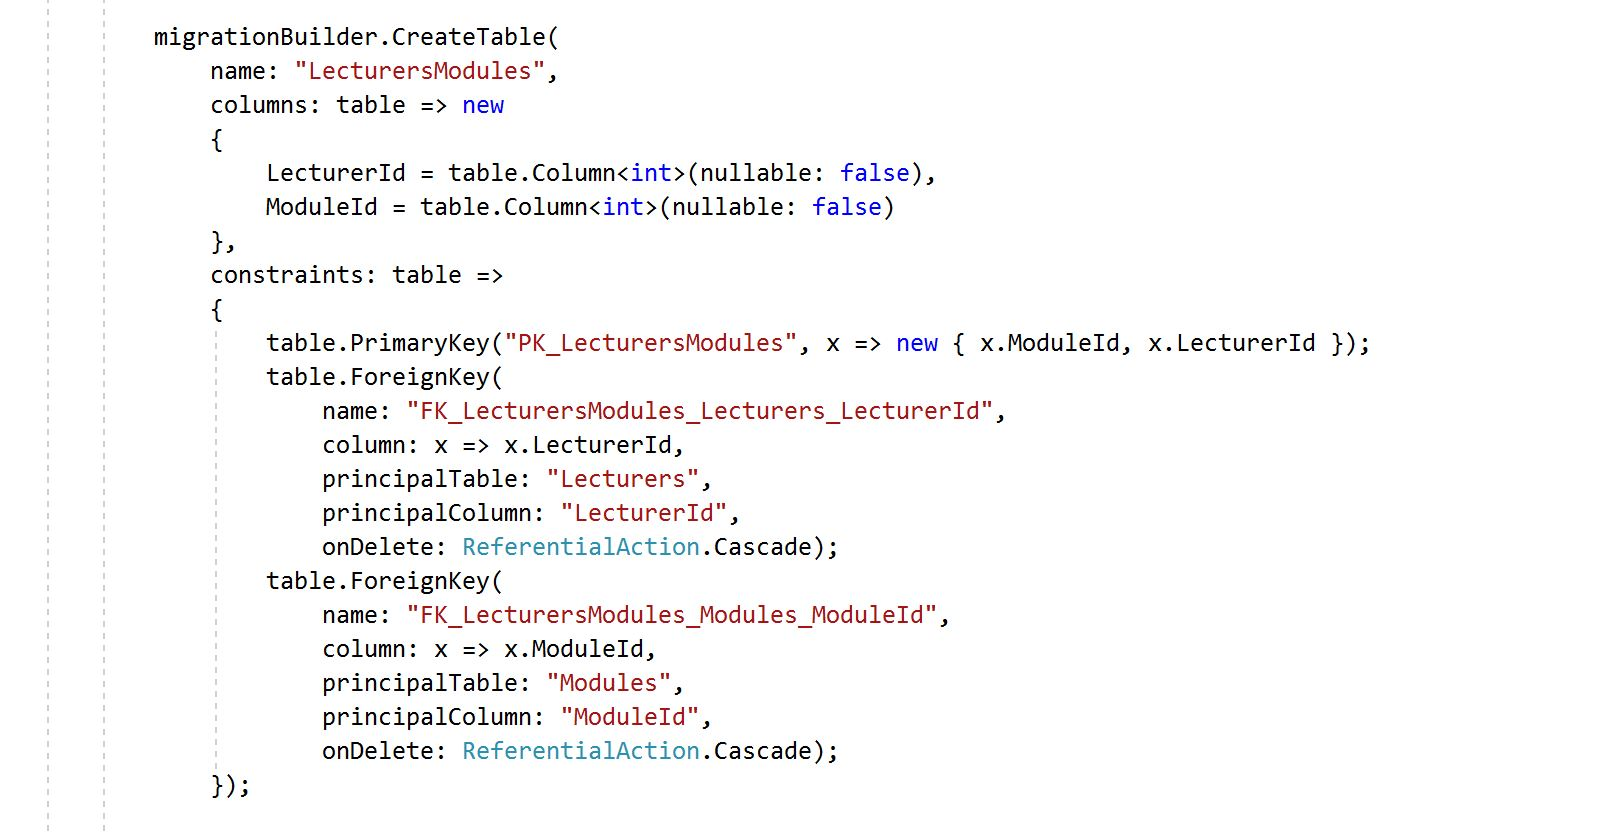
\includegraphics[width=150mm]{report_img/Initial.JPG}
\caption{Initial Migration File}
\label{blabla}
\end{figure} 

From Figure 3 we can see that one many-to-many relationship has transformed in two one-to-many and many-to-one relationships.

\begin{figure}[H]
\centering
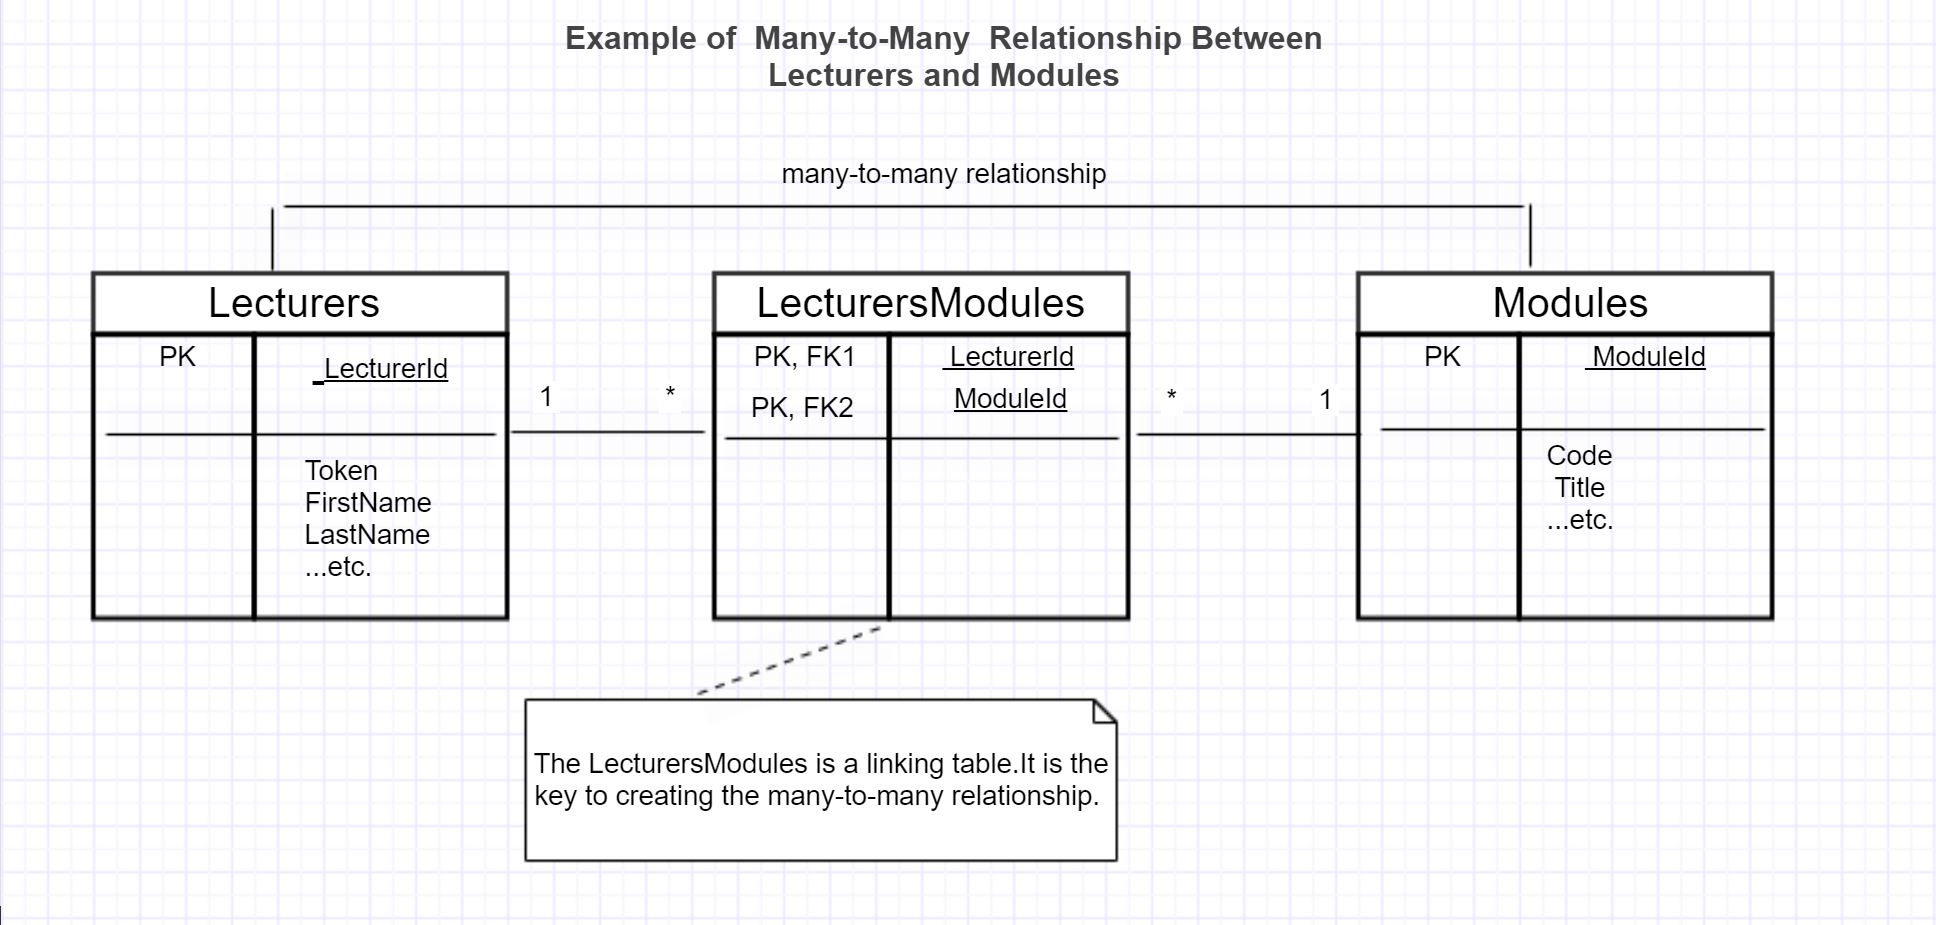
\includegraphics[width=150mm]{report_img/many-to-many-tables.JPG}
\caption{Creating Many-To-Many Relationship}
\label{blabla}
\end{figure}



\subsection{Creating Database}
\newpage
\subsection{Creating a Repository}

todo: photo of repository



In our project we create a repository interfaces and implementation classes.\\
We use \textbf{IQueryable<T> and IEnumarable<T>} interfaces.
With IQueryable<T> interface the objects can be queried in more efficient way.\\
For example: \textbf{public IQueryable<ModuleRun> ModuleRuns => appDbContext.ModuleRuns;} the ModuleRuns property in the context class returns a DbSet<ModuleRun> object, which implements the IQueryable<T> interface.

\noindent                                                                %
\begin{minipage}{\linewidth}                     
\makebox[\linewidth]{                                      
  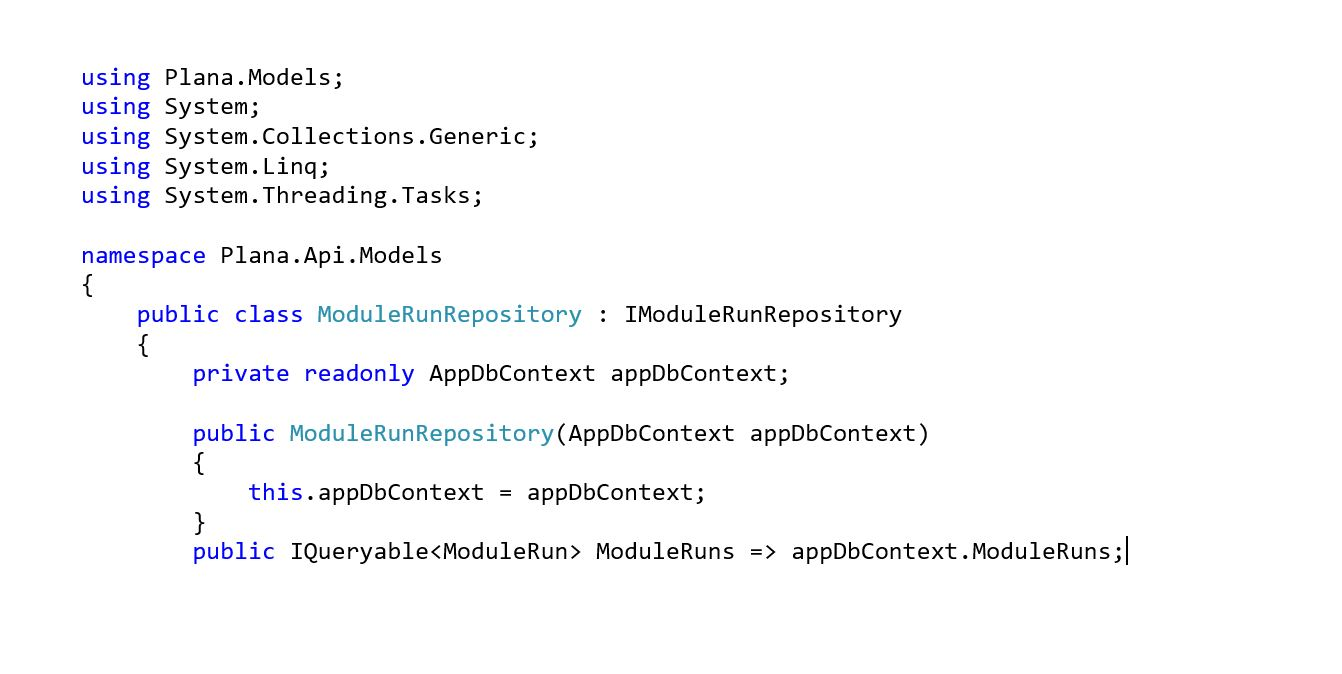
\includegraphics[keepaspectratio=true,scale=0.9]{report_img/repo-create.JPG}}
\captionof{figure}{The ModuleRunRepository.cs file in the Plana.Api/Models folder}
%\label{visina8                                                      }%  only if needed  
\end{minipage}


\newpage

Then we create the Repository Service in the Startup.cs file.\\

\begin{figure}[h]
\centering
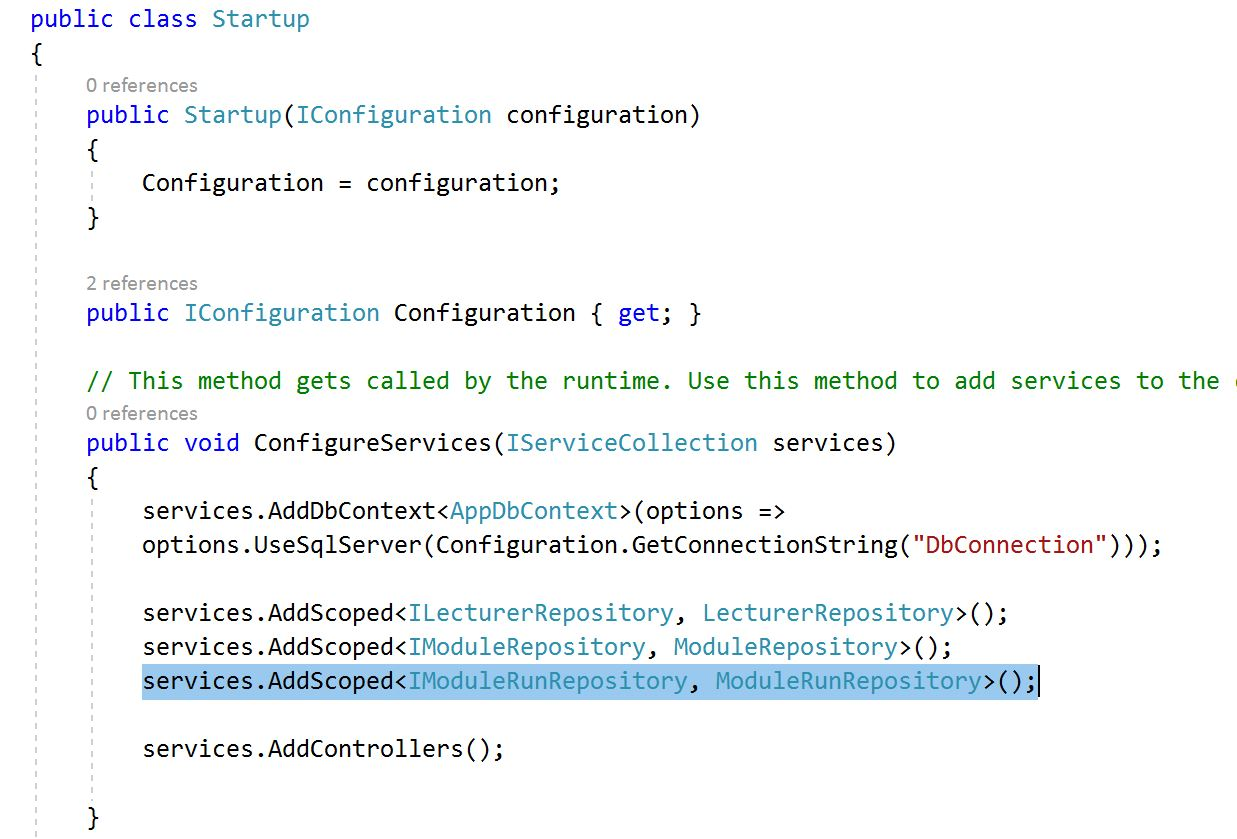
\includegraphics[width=150mm]{report_img/add_scoped_rep.JPG}
\caption{Creating Services in Startup.cs File}
\label{blabla}
\end{figure}

 

\cite{core3}

\subsubsection{Creating the Database Migration, Code-First Migration}
Entity Framework Core makes it possible to generate schema for the database from the data model classes using \textbf{migrations}
\textbf{dotnet em migrations add Initial} 
\cite{core3}



\subsection{Creating Seed Data}
The seed data is the data that is used to populate the database. For seed data we add class SeedData.cs in the Models folder in Plana.Api project \cite{core3}.
%\subsubsection{Delete method in Entity Framework Core}
By default, Entity Framework Core uses cascade deletes for depend relationships with non-nullable foreign keys. \cite{efa} \\
..add photo of seed class (give it name The contents of the SeedData.cs class \\
\subsubsection{Configuration of Core Services and Entity Framework}

It is necessary to make changes in Startup.cs class in Plana.Api project - configure Entity Framework Core and set up the services that will be used to access the database \cite{efa}.\\
The figure below shows all these configurations.

\noindent%
\begin{minipage}{\linewidth}% to keep image and caption on one page
\makebox[\linewidth]{%        to center the image
  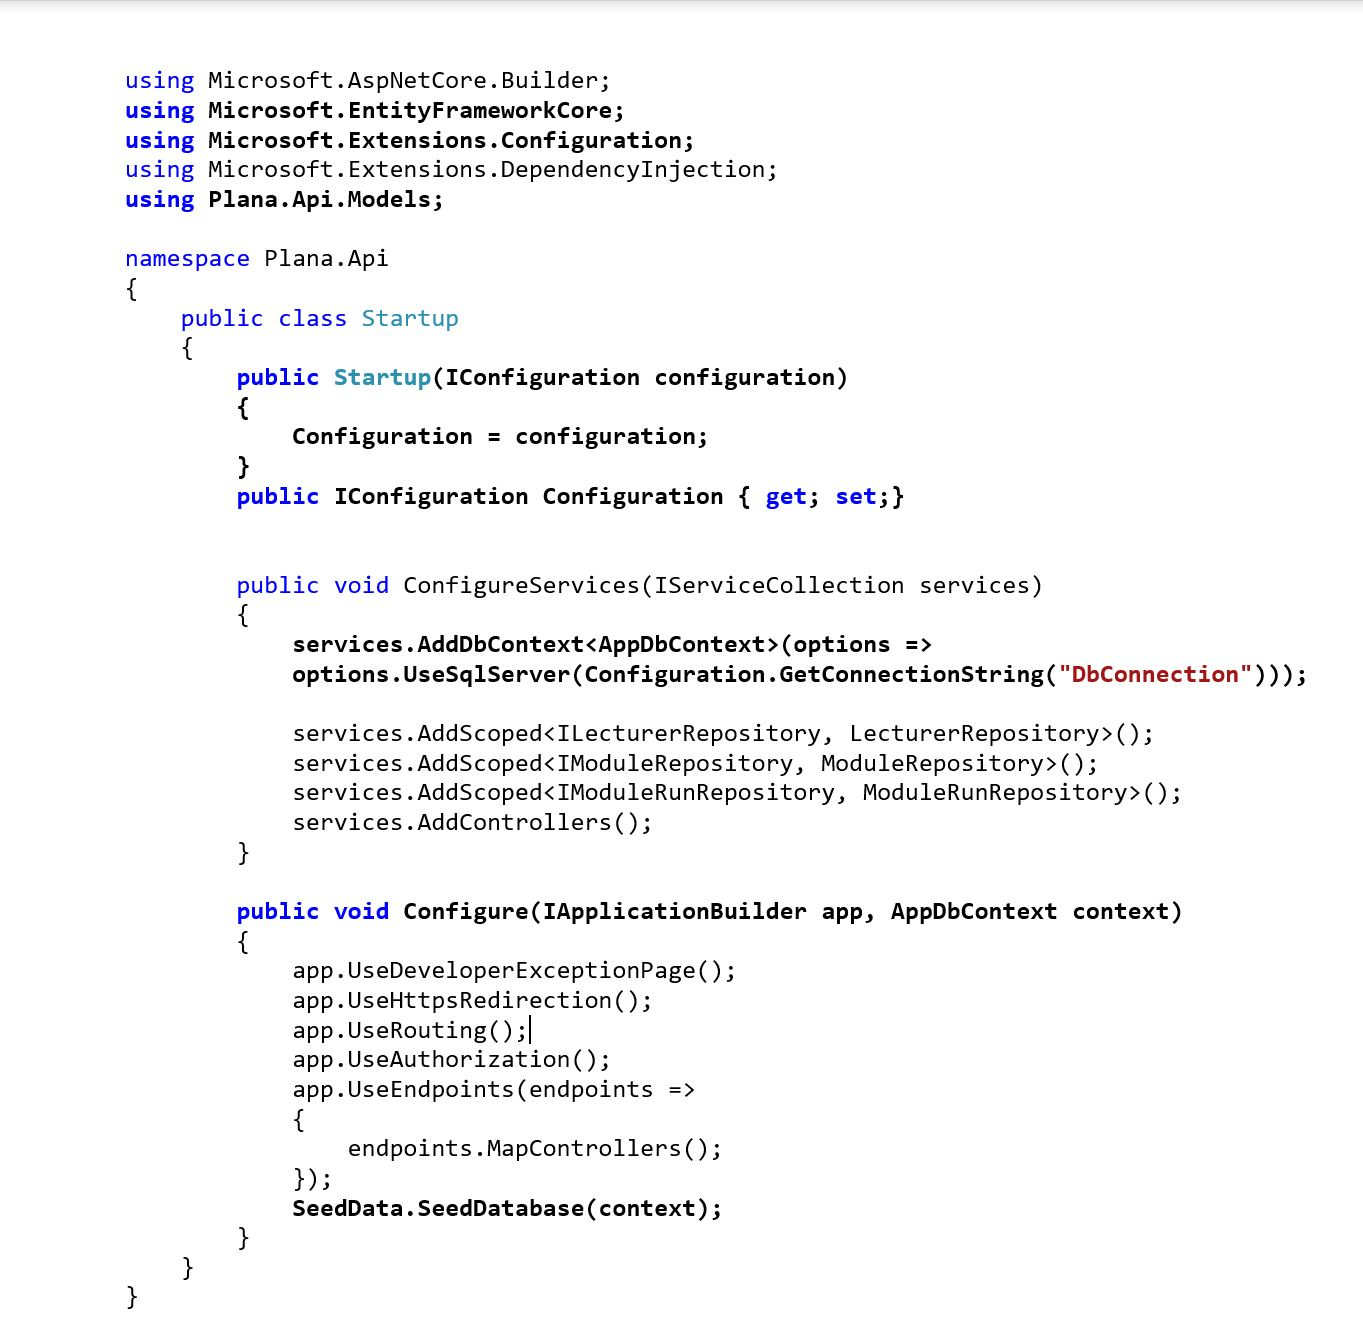
\includegraphics[keepaspectratio=true,scale=0.8]{report_img/seed-data-startup.JPG}}
\captionof{figure}{Startup.cs in the Plana.Api project.Preparing Services and Middleware}
%\label{visina8}%      only if needed  
\end{minipage}


\subsection{Create an Controller}

















%\section{Technologies}


\subsubsection{Complex Data Model}
in this section I would like to highlight more complex features of coding and data model structure in asp .net core.\\

\noindent                                                                %
\begin{minipage}{\linewidth}                            % to keep image and caption on one page
\makebox[\linewidth]{                                       %  to center the image
  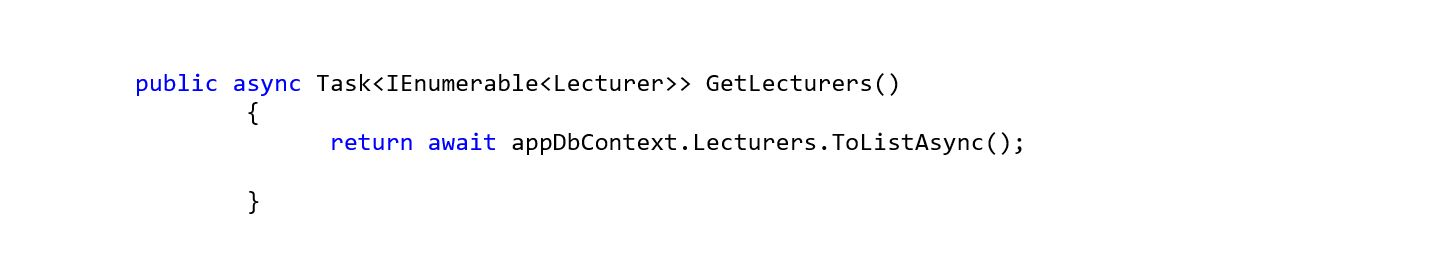
\includegraphics[keepaspectratio=true,scale=0.9]{report_img/complex_data_problem/repository_get_lecturers}}
\captionof{figure}{LecturerRepository.cs file in the Plana.Api project's folder}
\label{visina8                                                      }%  only if needed  
\end{minipage}



\begin{figure}[H]
\centering
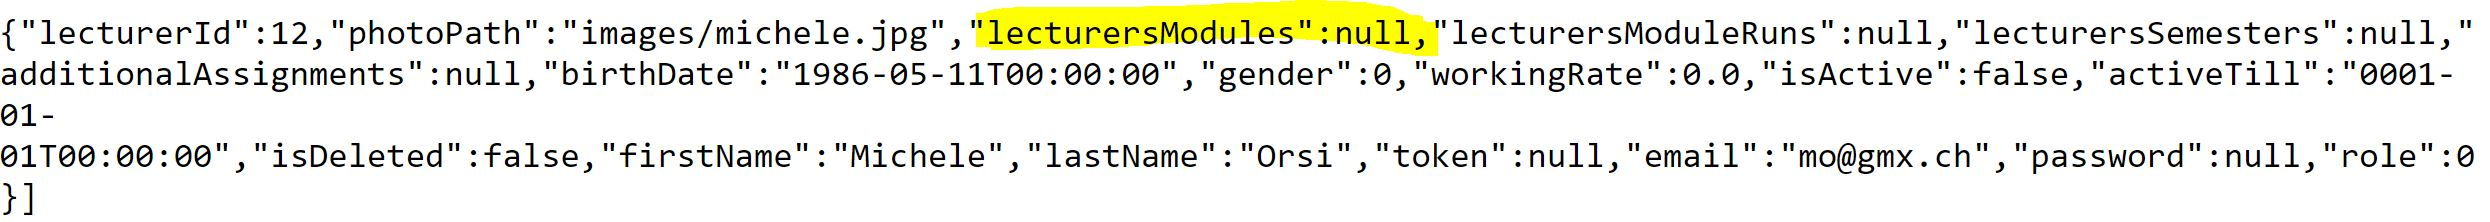
\includegraphics[width=150mm]{report_img/complex_data_problem/michele_module_null}
\caption{}
\label{blabla}
\end{figure}

\noindent                                                                %
\begin{minipage}{\linewidth}                            % to keep image and caption on one page
\makebox[\linewidth]{                                       %  to center the image
  
\includegraphics[keepaspectratio=true,scale=0.9]{report_img/complex_data_problem/repository_get_lecturers_modules}}
\captionof{figure}{...}
\label{visina8                                                      }%  only if needed  
\end{minipage}




\begin{figure}[H]
\centering
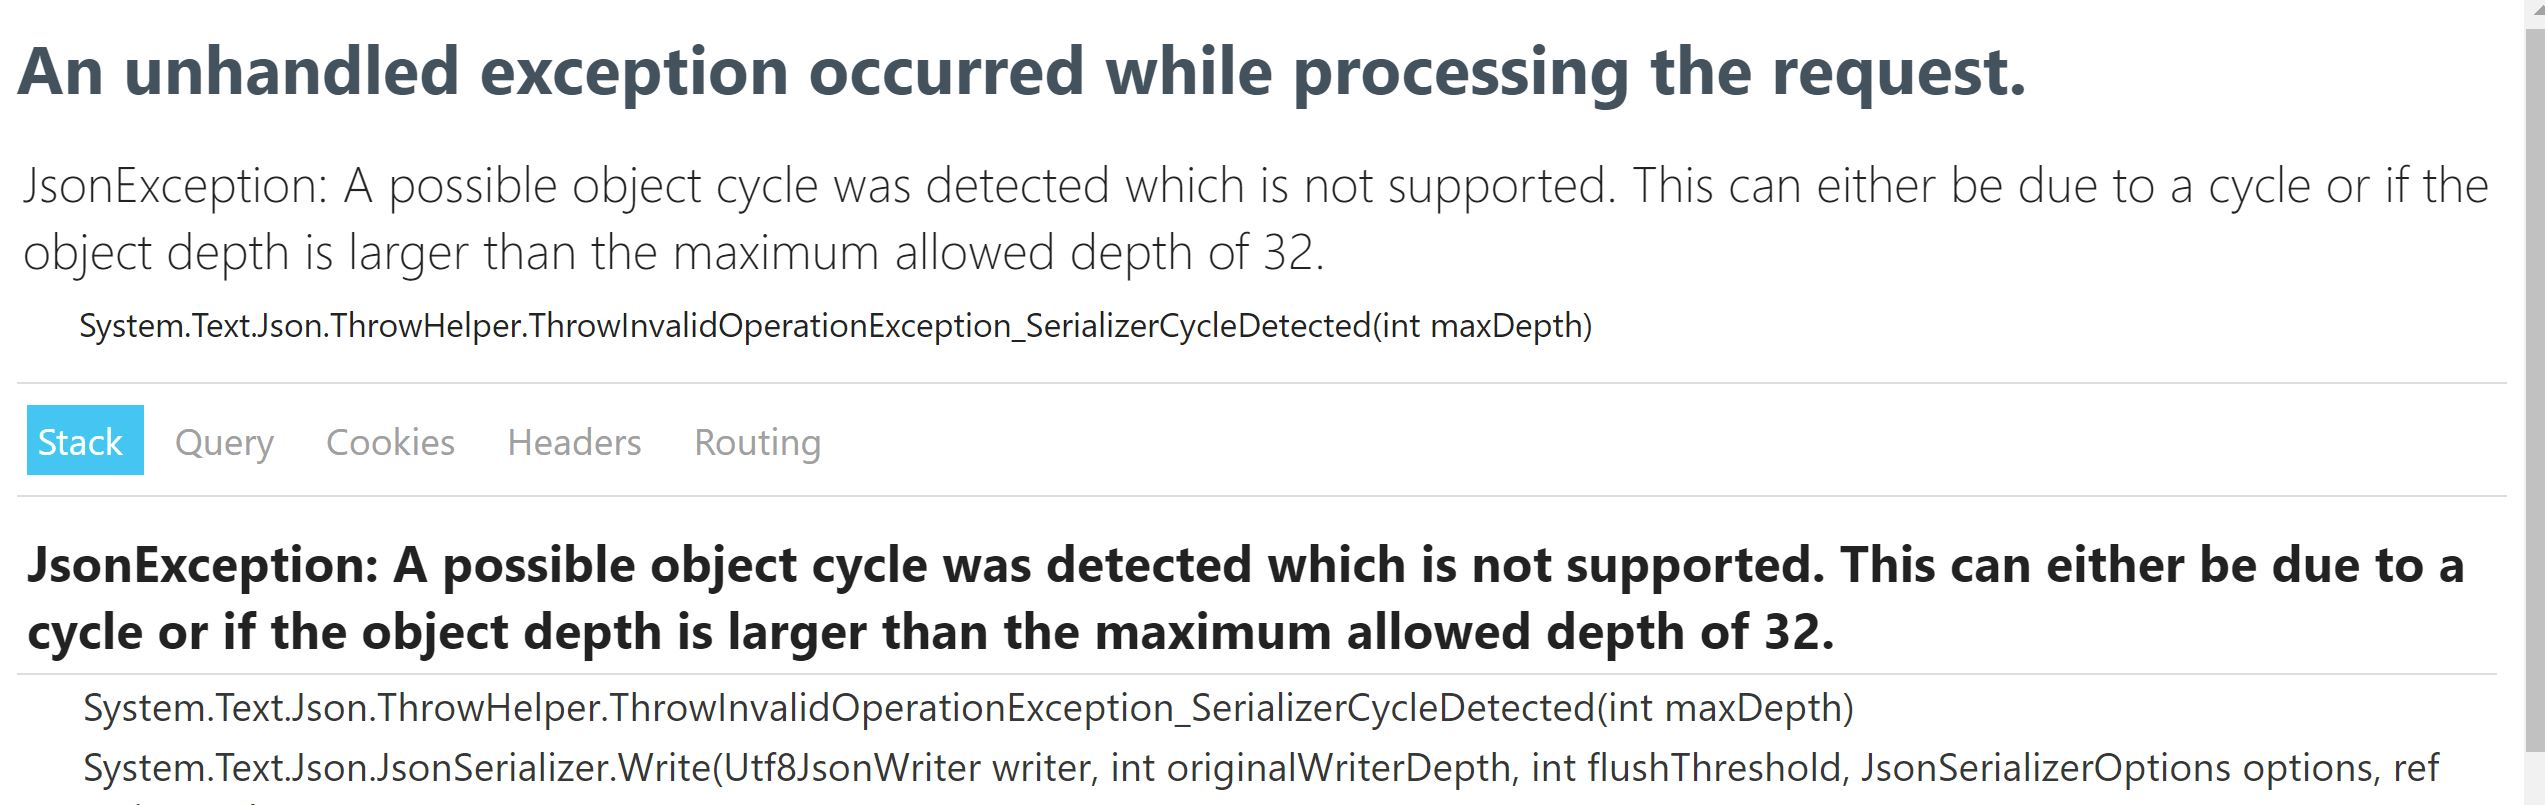
\includegraphics[width=150mm]{report_img/complex_data_problem/json_problem}
\caption{}
\label{blabla}
\end{figure}

\begin{figure}[H]
\centering
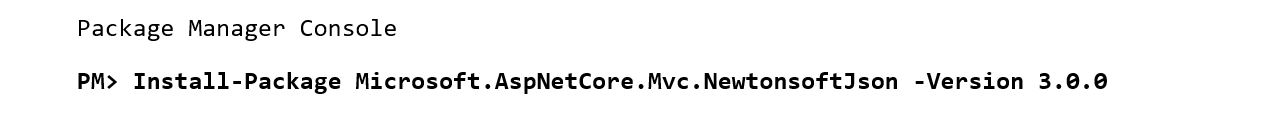
\includegraphics[width=150mm]{report_img/complex_data_problem/install_newtonsoft_json}
\caption{}
\label{blabla}
\end{figure}

\noindent                                                                %
\begin{minipage}{\linewidth}                            % to keep image and caption on one page
\makebox[\linewidth]{                                       %  to center the image
  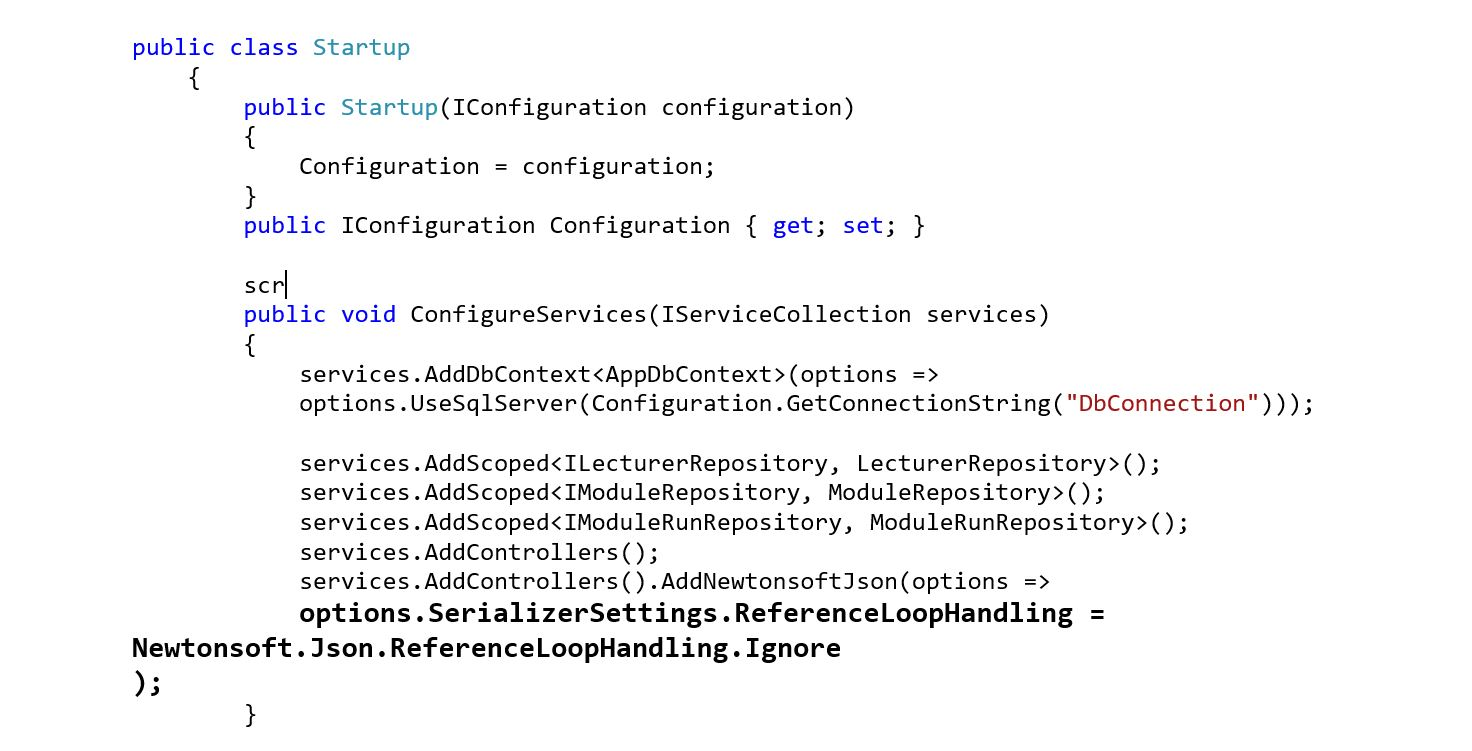
\includegraphics[keepaspectratio=true,scale=0.9]{report_img/complex_data_problem/startup_add_newtonsoft}}
\captionof{figure}{...}
\label{visina8                                                      }%  only if needed  
\end{minipage}




\begin{figure}[H]
\centering
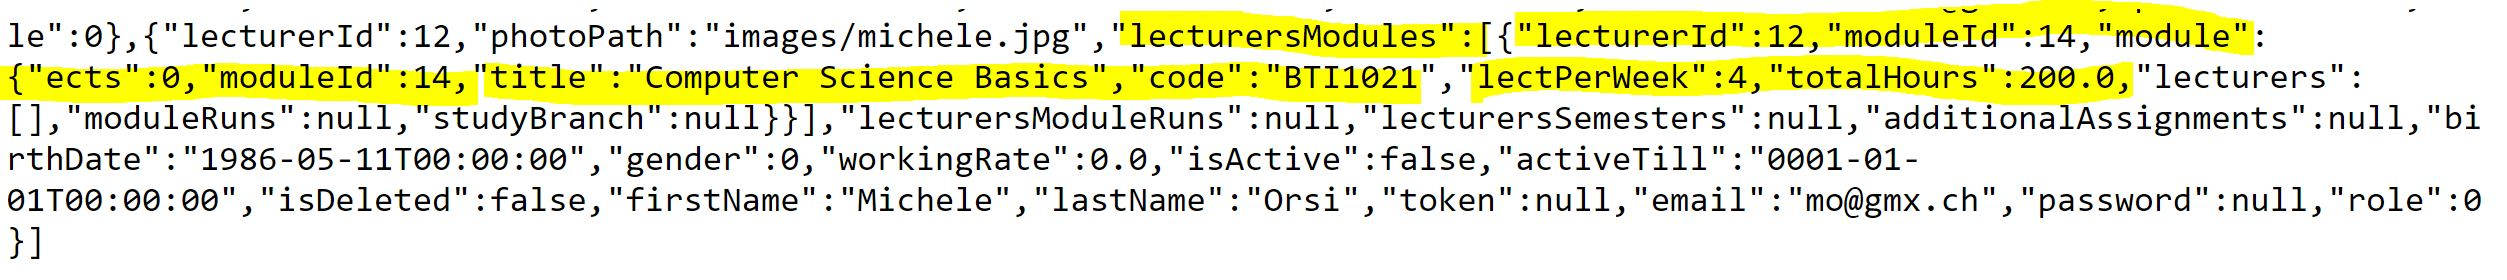
\includegraphics[width=150mm]{report_img/complex_data_problem/michele_module_ok}
\caption{}
\label{blabla}
\end{figure}

\subsection{Setup for Blazor}
To use the Blazor framework it is necessary to install :\\
\begin{itemize}
\item \textbf{.NET Core SDK 3.1 or later} from \url {http://dotnet.microsoft.com/download}
\item \textbf{Visual Studio 2019} from \url {https://visualstudio.microsoft.com/downloads/}
\end{itemize}

%\section{Proof of Concepts }
%/**
%determine whether an idea can be turned into a reality\\
%test if the idea is viable and explore 
%\\
%how the proposed product or service will support organizational goals\\
%*/







\section{Work Plan}
  		\subsection{Effort Estimation}
  		
  		The Bachelor's Thesis  is designed as a 12 ECTS module. This corresponds to a workload of 360 hours. When we are working on a project, we always record our hours of work in an Excel table.
 At the end of the project, we will compare this time with the time allotted for the project. 		
  		
  		
  		
  		
  		
 	    \subsection{Scrum}  	
 	    The foundation of the project organization was Scrum.
 	    Some principles of Scrum could not be achieved since they need a group of more than two people. 
 	    Our work was based on the principles of Scrum like the Empirical Process of Control, the core of Scrum, self-organization, value-based prioritization, etc.
 	    The Empirical Process of Control includes three main ideas, namely transparency, inspection, and adaptation. \\
 	    Transparency: The work is carried out in full trust of all parties involved. Everyone has the courage to keep each other up to date with both good and bad news. \\ 
 	    Inspection: Inspection is carried out by every one in the Scrum Team. The team openly shows the product at the end of each Sprint.			 \\
 	    Adaptation: The team asks constant questions about the progress of work, whether we are on the right way. Depending on this, we can adapt an existing product.		 \\
 	    
 	    At the beginning of the project, we have discussed and estimated all the work that needs to be done. 
 	    Meetings between supervisor and developer are weekly and sometimes bi-weekly.
 	    Each meeting includes a discussion about what has been achieved 
 	    since the tasks have been assigned, what can be improved, and scheduling of future tasks.
 	    
 	    
 	    
 	    
 	    
  		\subsubsection{Scrum Roles}
  		\begin{itemize}
  		\item Product Owner: Mr. Pfahrer
  		\item Development Team: Shiryagina Kristina
  		\item Scrum Master: Shiryagina Kristina
  		
  		\end{itemize}
  	    \subsubsection{Scrum Plan}
  	    To discuss the project, were weekly and biweekly meetings held . They included personal meetings, and then meetings using Microsoft Teams. The meetings consisted of:
  	    \begin{itemize}
  	    \item Sprint Review. It includes a show of work and its discussion.
  	    \item Sprint Planning. It includes the scheduling of future tasks.
  	    \item Sprint Retrospective. It includes discussion about what went well and what went wrong, what we should do differently. 
  	    \end{itemize}
  		\subsubsection{Scrum Artifacts }
  		
  		\subsubsection{Sprints}
  		
	The sprints covered a one three-four weeks period. At the end of each sprint, there was a discussion with the supervisor.
%
%In Table 11 is an overview of what was achieved in which sprint.
%\textbf{Sprint's Backlog}
%
%\begin{table}[H]
%\begin{center}
%\begin{tabular}{| p{1cm}|p{3cm}|p{7.5cm}|p{2.5cm} |p{2.5cm} |}
%\hline
%\rowcolor{LightCyan}
%\textbf{ID} & \textbf{Task Name} & \textbf{Task Description}  & \textbf{Priority} & \textbf{Status}\\
%\hline
%
%1                   &        & & & trtwt      
%\begin{itemize}
%\item 
%\item
%\item
%
%
%
% \end{itemize}\\ \hline
% 
%2                &     & & &                
%\begin{itemize}
%\item 
%\item
%\item
%
%
% \end{itemize}\\ \hline
% 3                 &     & & &                  
%\begin{itemize}
%\item 
%\item
%\item
%
%
% \end{itemize}\\ \hline
% 4                  &     & & &               
%\begin{itemize}
%
%\item 
%\item
%\item
%\end{itemize}\\ \hline
% 
%  5            &     & & &                 
%\begin{itemize}
%
%\item 
%\item
%\item
%
% \end{itemize}\\ \hline
% 
%
% 
% 
%
% \end{tabular}
%\end{center}
%\caption{Sprint Backlog of Sprints}
%\label{table2}
%\end{table}
%
%\pagebreak
%
%\begin{table}[H]
%\begin{center}
%\begin{tabular}{| p{1cm}|p{3cm}|p{7.5cm}|p{2.5cm} |p{2.5cm} |}
%\hline
%\rowcolor{LightCyan}
%\textbf{ID} & \textbf{Task Name} & \textbf{Task Description}  & \textbf{Priority} & \textbf{Status}\\
%\hline
%
%6                &     & & &        
%\begin{itemize}
%\item 
%\item
%\item
%
%
% \end{itemize}\\ \hline
% 
%  7                &     & & &                 
%\begin{itemize}
%\item 
%\item
%\item
% \end{itemize}\\ \hline
% 
%  8                 &     & & &                 
%\begin{itemize}
%\item 
%\item
%\item
%
%\end{itemize}\\ \hline
%
%  9                 &     & & &                  
%\begin{itemize}
%\item 
%\item
%\item
% 
%\end{itemize}\\ \hline
% 
%  10               &     & & &                 
%\begin{itemize}
%\item 
%\item
%\item
%
%
% \end{itemize}\\ \hline
% 
%  11                &     & & &                 
%\begin{itemize}
%\item 
%\item
%\item
%
% \end{itemize}\\ \hline
% 
% 
% \end{tabular}
%\end{center}
%\caption{Sprints}
%\label{table2}
%\end{table}
% 
% 
% \pagebreak
%\begin{table}[H]
%\begin{center}
%\begin{tabular}{| p{1cm}|p{3cm}|p{7.5cm}|p{2.5cm} |p{2.5cm} |}
%\hline
%\rowcolor{LightCyan}
%\textbf{ID} & \textbf{Task Name} & \textbf{Task Description}  & \textbf{Priority} & \textbf{Status}\\
%\hline
% 
%  12               &     & & &                  
%\begin{itemize}
%\item 
%\item
%\item
% 
%
% \end{itemize}\\ \hline
% 
%  13                &     & & &                  
%\begin{itemize}
%\item 
%\item
%\item
%
%
% \end{itemize}\\ \hline
%  14               &     & & &                   
%\begin{itemize}
%\item 
%\item
%\item
%\end{itemize}\\ \hline
% 
% 15                 &     & & &                  
%\begin{itemize}
%
%\item 
%\item
%\item
%
%
% \end{itemize}\\ \hline
% 16               &     & & &                  
%\begin{itemize}
%\item 
%\item
%\item
%
%
% \end{itemize}\\ \hline
% 17               &     & & &                   
%\begin{itemize}
%\item 
%\item
%\item
%
% \end{itemize}\\ \hline
% 
%\end{tabular}
%\end{center}
%\caption{Sprints}
%\label{table2}
%\end{table}



\section{Conclusions and Future Work}
%   \subsubsection{Summary}
\subsection{Conclusions}
   
    	\subsection{Future Work		}
    	


\newpage

%% print the bibliography and add the section to the table of content

\printbibliography[heading=bibintoc]


\pagebreak









  	
  
  	

  	
  	
  	
  
  	
  	
  	
  
  	
  	
  
  	


  	





	
	
	




 









 

 























                      
        
    


   

   
    
   
  

\section{Protocol}
\textbf{\textit{Frequency: (weekly) \\
Meeting length: (60 minutes)}}\\

Agenda

\begin{itemize}
  	\item Demo and Discuss Deliverable(Demo)
  	\item Planning next Goals(Plan)
  	\item Lessons learned (Lessons)
  	\item Date, time of the next meeting(next meeting)
 \end{itemize} 	


\textbf{\textit{Report from   }}\\
Plan\\
Future goals are: 
\begin{itemize}


	\item 
	\item 
\end{itemize}	
Lessons learned\\

Next Meeting: .....\\
%%%%%%%%%%%%%%%%%%%%%%%%%%%



%%%%%%%%%%%%%%%%%%%%%%%%%%%%





\end{document}





